% !TeX encoding = UTF-8
% !TeX program = pdflatex

\documentclass[12pt]{article}
\usepackage{hyperref}
\usepackage{graphicx}
\usepackage{listings}
\usepackage{amsmath}
\usepackage{verbatim}

\usepackage{pgfplots}
\pgfplotsset{compat=1.14}

\hypersetup{
 colorlinks,
 citecolor=black,
 filecolor=black,
 linkcolor=black,
 urlcolor=black
}

\renewcommand{\baselinestretch}{1.15}

\title{{\bf Compiler Provenance} \\ \bigskip \large HW1 - Machine Learning \\ \large "Sapienza" University of Rome}
\author{Valerio Coretti 1635747}
%\pagenumbering{roman}

\begin{document}
\maketitle

\begin{abstract}

Nowadays the amount of malicious programs is increasing exponentially and the number of victims is very high. For this reason, Malware Analysis is a crucial point in Cybersecurity.

Machine Learning plays a key role in malware analysis because it can simplify various processes in several ways. The goal of an analyst is to capture malicious aspects and traits having the broadest scope, and Machine Learning is a natural choice to support this process of knowledge extraction.

In this project, we use Machine Learning techniques to simplify the problem of Reverse Engineering of malware. When an analyst has a new malware sample to analyze, the first thing to do is to disassemble it. This permits the analyst to look at the binary code of all the functions contained inside the malware. The problem is that a human cannot analyze all the code but he tries to focus on a specific part of the sample that for some reason looks more interesting. But in most cases, malware binaries are often stripped or the string inside a binary can be encrypted. In this scenario, an automated approach is a good way to reverse malware binaries.

There are several problems in binary analysis, one of these is the {\em Compiler Provenance}.

{\em Problem}: given the binary code of a function, which are the compiler and the optimization who produced it?

To address this problem, Machine Learning is used with notable results.

In this paper, we will discuss an approach based on {\em Supervised Learnin} and we will try to solve these two classification problems.

\end{abstract}

\section{Introduction}
We have two problems: {\em Optimization Detection} and {\em Compiler Detection}.
To solve these problems with Machine Learning we analized a large dataset that is a ".jsonl" file that contains 30000 functions. Each row of the file is a json object like that:
\begin{quote}
$\{$
 \newline
 {\em "instructions"}: ["xor edx edx", "cmp rdi rsi", "mov eax dword [localch]", "seta dl", "cmovae eax edx", "ret"],
 \newline
 {\em "opt"}: "H",
 \newline
 {\em "compiler"}: "gcc "
 \newline
$\}$
\end{quote}

The first problem is a Binary Classification problem because we have only two types of optimization: High or Low.
Instead the second is a Multiclass Classification problem and we have three classes of compiler: gcc, icc, clang.

The compiler distribution is very {\em balanced}, we have 10000 functions per compiler, while the optimizations distribution
is {\em unbalanced}, we have 17924 low and 12076 high.

What we will see in the following sections is a description of what we did to solve these problems.
We will begin by illustrating how we transformed the dataset up to which model we have definitively chosen. By doing this we explored two ways of features extraction and compared three types of models:
{\em Bernoulli Naive Bayes},
{\em Multinomial Naive Bayes},
and finally {\em Support Vector Machine with Linear kernel}.

We worked with {\em Scikit-Learn} that is a simple and efficient Python OpenSource tool for data mining and data analysis.

\section{Preprocessing}
The solution we thought is similar to text analysis, and we based our idea on the Spam Classification Problem.
Therefore we have done some operations to transform the dataset for our purpose. Given a function (equivalent to a row) we have transformed the instruction set into a single string. Such as:
\begin{quote}
{\em "instructions"}: ["xor edx edx", "cmp rdi rsi", "mov eax dword [localch]", "seta dl", "cmovae eax edx", "ret"]
\end{quote}
\centerline{becomes}
\begin{quote}
{\em "instructions"}: ["xor edx edx cmp rdi rsi mov eax dword [localch] seta dl cmovae eax edx ret"]
\end{quote}


\subsection{Thinning dataset}
The main difference with the spam problem is that we have transformed the dataset of the functions in such a way as not to take all the instructions and operands inside, but limiting ourselves to taking the {\em mnemonics} of the assembly instructions and, in addition, we have selected {\em memory accesses} and {\em register accesses}. These choices are justified by the fact that the set of all instructions is unbounded but if we consider only mnemonics the set is smaller. Memory and register accesses are important because when a compiler optimizes a function it tries to reduce the memory accesses and to use as much as possible the registers, which are faster than the memory.

To extract memory accesses we based on four key word:
\begin{itemize}
\item {\em "qword", "dword", "word", "byte"}
\end{itemize}
This commands mean: {\em "take n bytes from a certain data segment"}.
Instead for registers we choosed the main ones:
\begin{itemize}
\item Data Registers: {\em "eax", "ebx", "ecx", "edx"}
\item Pointer Registers: {\em "ebp", "esp"}
\item Index Registers: {\em "edi", "esi"}
\end{itemize}

Done this, the previous example becomes:
\begin{quote}
{\em "instructions"}: ["xor edx edx cmp rdi rsi mov eax dword seta dl cmovae eax edx ret"]
\end{quote}

Now we are ready for the extraction of the features.

\subsection{Features Extraction}
The list of features can be processed like a list of words in a document. For this reason we use a sklearn vectorizer. The power of a vectorizer is that it not take only term by term (called 1-grams mode) but it can also keep the word order in a text by making more words a single feature. This function is called n-grams. For example for 1-grams if we have only the previous seen string the features is every single word in the string itself, but if we set the range of n-grams at (1, 3) we will have:
\begin{quote}
['cmovae', 'cmovae eax', 'cmovae eax edx', 'cmp', 'cmp rdi', 'cmp rdi rsi', 'dl', 'dl cmovae', 'dl cmovae eax', 'dword', 'dword seta', 'dword seta dl', 'eax', 'eax dword', 'eax dword seta', 'eax edx', 'eax edx ret', 'edx', 'edx cmp', 'edx cmp rdi', 'edx edx', 'edx edx cmp', 'edx ret', 'mov', 'mov eax', 'mov eax dword', 'rdi', 'rdi rsi', 'rdi rsi mov', 'ret', 'rsi', 'rsi mov', 'rsi mov eax', 'seta', 'seta dl', 'seta dl cmovae', 'xor', 'xor edx', 'xor edx edx']
\end{quote}

In our project as a first attempt, we try with 1-grams mode but as we will see it not perform very well, then swapping to (1, 3)-grams we have achieved pretty results. Note that, as you can see from the output, for a very large dataset the number of features, with (1, 3)-grams, can be a very high number, for this reason, we only consider the top 10000 features ordered by term frequency across the corpus.

Furthermore, for the extraction, we choose a precise vectorizer: {\em Tf-Idf Vectorizer}. This object converts a collection of raw documents into a matrix of TF-IDF features. Tf-idf is the short form of {\em term frequency-inverse document frequency}, it doesn't count the recurrence of a word in a certain row but is a numerical statistic that reflects how important a word is in a document.

The function can be split into two factors: the first factor of the function is the number of terms in the document. In general, this number is divided by the length of the document to prevent longer documents being privileged.

\bigskip
$tf_{i,j} = \displaystyle \frac {n_{i,j}}{|d_j|} $
\bigskip

where $n_{i,j}$ is the number of occurrences of the term {\em i} in the document {\em j}, while the denominator is simply the size, expressed in the number of terms, of the document {\em j}.

The other factor of the function indicates the general importance of the term {\em i} in the collection:

\bigskip
$idf_{i} = log \displaystyle \frac {|D|}{|\{ d : i \in d \}|} $
\bigskip

where $|D|$ is the number of documents in the collection, while the denominator is the number of documents containing the term {\em i}

Therefore we have:

\bigskip
$(tf-idf)_{i,j} = tf_{i,j} * idf_{i}$
\bigskip

Now we have our structure. The last important thing to do is divide the dataset into two parts, one for the training and one for the evaluation. The training set is 2/3 of the original dataset and the evaluation set is the remaining 1/3. We decided also to keep the proportion of the classes the same in both problems.

This division is performed by choosing random elements, so running different times the preprocessing phase will affect the final results a bit.

\section{Model}
To get to the final result we explored three different models: {\em Bernoulli Naive Bayes}, {\em Multinomial Naive Bayes}, and finally {\em Support Vector Machine with Linear kernel}. In the following sections, we explain how these models work and then we will discuss the evaluation.
\subsection{Naive Bayes Classifiers}
The first chosen model is the {\em Naive Bayes classifier}, a probabilistic model used mainly for text classification. In this model, a document is viewed as a collection of words. As we said before the list of features can be processed like a list of words in a document without losing information, so this model is suitable for our problem.

In our case we divided the problems, in the first we have two classes $c_1$ and $c_2$, respcetively {\em High} and {\em Low} optimization, in the second we have three classes $c_1$, $c_2$ and $c_3$ as {\em "gcc"}, {\em "icc"} and {\em "clang"} .

We considered two variants of Naive-Bayes, the {\em Bernoulli} and the {\em Multinomial}.

The Naive-Bayes model classifies an instance $x$, represented as a set of features $<x_0 ... x_n>$, with the class $c_m$ which maximizes the probability $P (c_m | x, D)$, where $D$ is the dataset.
The class is computed using the following function:

\bigskip
$argmax_{c \in C}\{P (c | x, D)\}$
\bigskip

that is equal to:

\bigskip
$argmax_{c \in C}\{P (x | c, D)P (c | D)\}$
\bigskip

And, assuming the conditional independece of the features (words) $x_i$, is also equal to:

\bigskip
$argmax_{c \in C}\{P (c | D) \Pi_i P (x_i | c,D)\}$
\bigskip

In the multinomial variant, this function becomes:

\bigskip
$argmax_{c \in C}\{ \displaystyle \frac{P(c | D) \Pi_i P(x_i | c, D)^{n_{x_i x}}}{P(x | D)}\}$
\bigskip

Where $n_{x_i x}$ is the number of times the word $x_i$ is in the document $x$.

$P(x_i|c, D)$ is defined in the following manner:

\bigskip
$P(x_i|c, D) = \displaystyle \frac{1 + \sum_{d \in D_c} n_{x_i d}}{k + \sum_{j} \sum_{d \in D_c} n_{x_j d}}$
\bigskip

With $D_c$ defined as the collection of documents in the training set of class $c$.
The additional $1$ and $k$ (the cardinality of the vocabulary) are the solutions to the zero-frequency problem.

\subsection{Support Vector Machine}
Here we are in the family of the Linear Classification Models. The basic idea of this type of models is that the instances in a dataset (e.g. binary) are {\em linearly separable} if exist a {\em linear function} (hyperplane) such that the instance space is divided into two regions, in one you find only positive examples in the other only negative ones. Support Vector Machine is a solution for the problem above and it is more sophisticated than the Naive Bayes.

SVM is a method in which we don’t want to find a line that divides instances simply, but which does it in the best way. We want a line that guarantees the maximum distance between points of the two classes from it.

So in Support Vector Machine we always look for 2 things:
\begin{itemize}
\item Setting a larger margin
\item Lowering misclassification rate
\end{itemize}
Now the problem is that these two things are kind of contradictory. If we increase margin, we will end up getting a high misclassification rate on the other hand if we decrease a margin, we will end up getting a lower misclassification rate. The answer is parameter C.

C is the penalty parameter of the error term. It controls the trade-off between smooth decision boundaries and classifying the training points correctly. Increasing C values may lead to overfitting the training data.

Another key point for a better use of SVM are the {\em Kernel functions}. These selects the type of hyperplane used to separate the data. Using {\em linear} kernel will use a linear hyperplane. Then we have kernel like {\em rbf} or {\em poly} that uses a 'non linear' hyperplane for the classification.
\begin{figure}[!ht]
 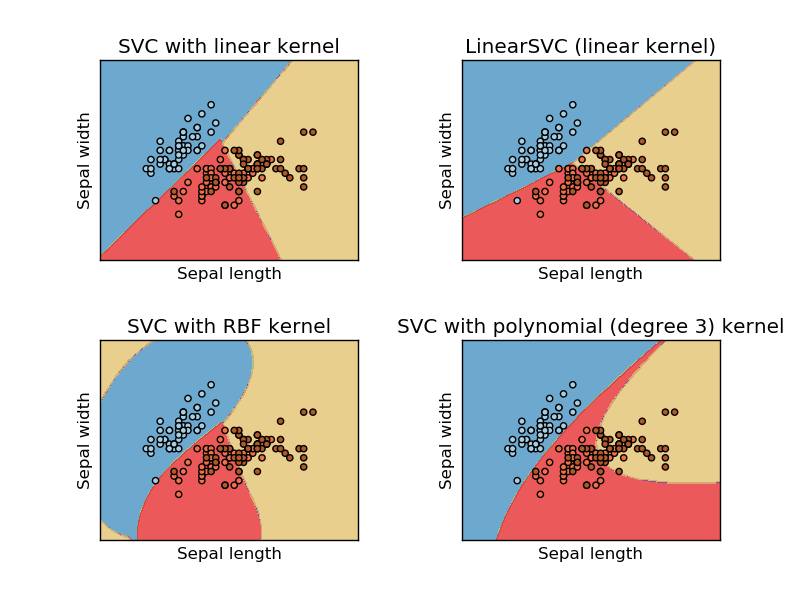
\includegraphics[width=1\textwidth]{pic1}
 \label{fig:Example of SVM}
\end{figure}
\newline
For our problem we use Support Vector Machine with Linear Kernel and for penalty parameter we set the standard value $C = 1$ because it give the best performance.

Now that we have a clearer overview of the methods we have used for our problem, we will discuss the evaluation of the results.

\section{Evaluation}
To perform a better classification, we evaluated the performance of training the model using two different features: {\em 1-gram} and {\em 3-grams}.

The output parameters that we considered for the evaluation are the following \footnote{Legend: TP = true positives, TN = true negatives, FP = false positives, FN = false negatives}:

\begin{itemize}
\item Precision: $TP / (TP + FP)$
\item Recall: $TP / (TP + FN)$
\item False positives rate: $FP / (FP + TN)$
\item False negatives rate: $FN / (FN + TP)$
\item Accuracy: $(TP + TN) / (TP + FN + TN + FP)$
\item F1-score: $ 2*(Recall*Precision)/(Recall+Precision)$
\end{itemize}

Furthermore we also based our analysis in the results posted by the {\em Confusion Matrix} that represents in each entry how many instances of class $C_i$
is misclassified as an element of class $C_j$. So, the main diagonal contains the true positive and true negative respectively for each class.
\begin{figure}[!ht]
 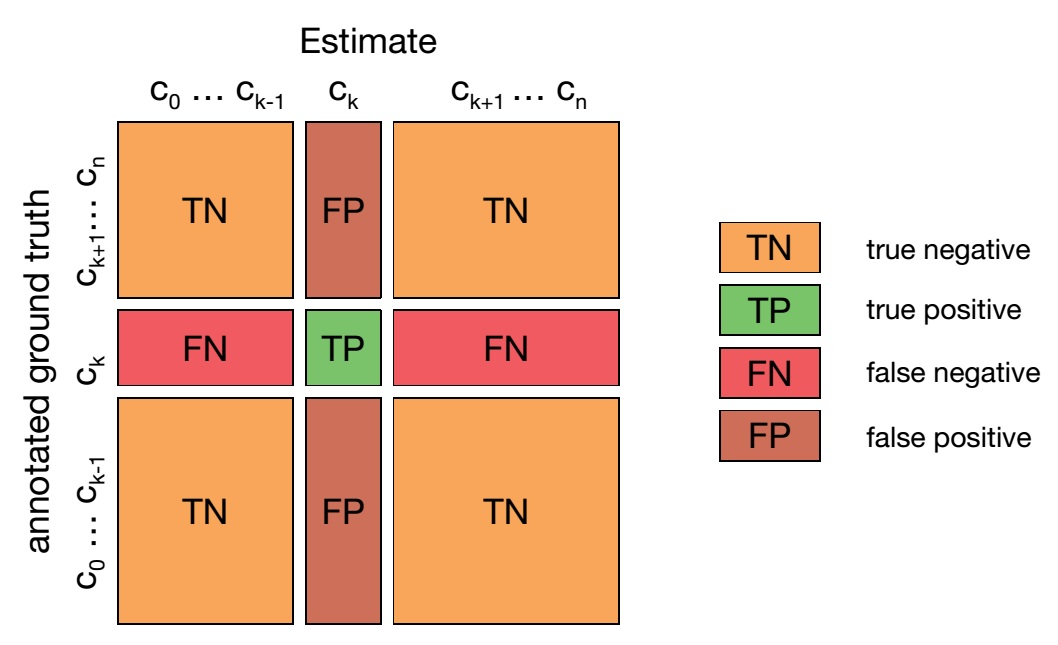
\includegraphics[width=1\textwidth]{pic2}
 \label{fig: Confusion Matrix}
\end{figure}
\newpage

In the following sections, we analyze the results and how we arrived at the final choice of the model. We divided the discussion, first we analyze the 1-gram feature and we will show why we decided to change strategy and use the 3-grams feature.

\subsection{1-gram feature}
This type of feature extraction takes only the words inside the functions and doesn't consider the order, for this reason, are very few, about 400 features. As a first attempt, we try with the Bernoulli Naive Bayes and Multinomial Naive Bayes. The results for our classification problems are the following:
\begin{figure}[!ht]
 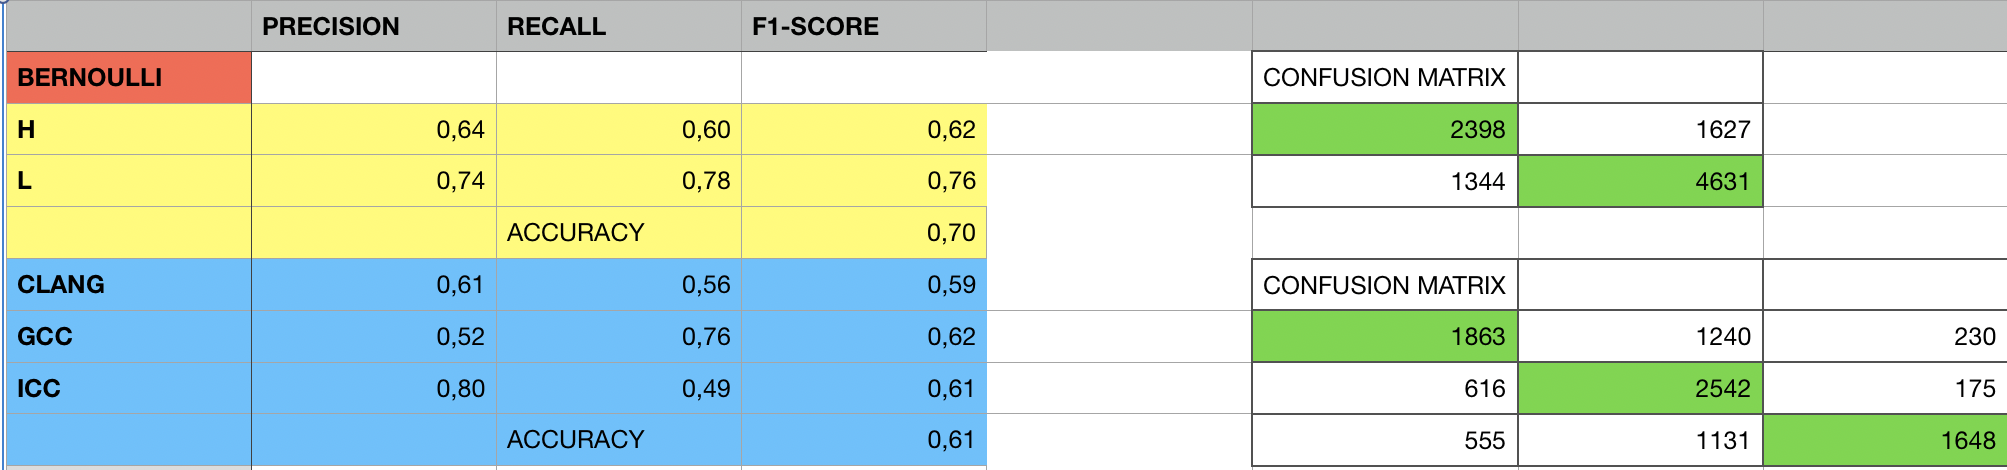
\includegraphics[width=1\textwidth]{pic3}
 \label{fig: Bernoulli with 1-gram}
\end{figure}

\begin{figure}[!ht]
 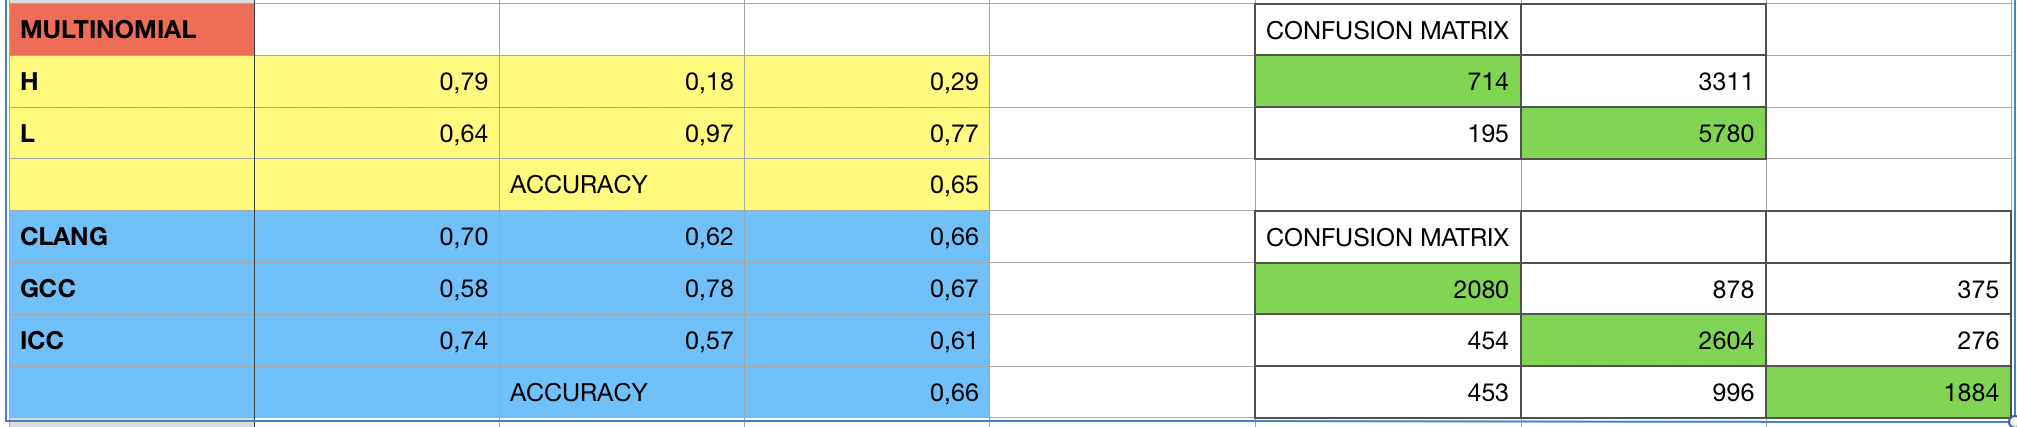
\includegraphics[width=1\textwidth]{pic4}
 \label{fig: Multinomial with 1-gram}
\end{figure}
\newpage

We stopped the experimentation here due to the very low accuracy. Note that the accuracy metric is not very effective for the evaluation of the optimization detection because we have an unbalanced distribution and for this reason, we pay more attention to the False Positive Rate and False Negative Rate. Besides, False Positive Rate is a key measure and must be maintained as low as possible.

These models with these features seem to classify a High optimization as a Low too often and also in the cases of the compiler detection the numbers of misclassification are very high.

Furthermore, as we can see in the picture above the results of the optimization classification with Multinomial are very bad because for the H class we have
$F1-score = 0,29$ and $Recall = 0,18$ this means that of all the functions that have an high optimization this model ranks very few.

To improve performance we first decided to improve features extraction and we analyze the results with the same models.

\subsection{3-grams feature}
This type of feature extraction making more words a single feature and consider the order, for this reason, the number of features is very high but we only consider the top 10000 features ordered by term frequency across the corpus.
In general, the multinomial variant is better than Bernoulli but we tried anyway to confirm this trend also for this case.
Using the multinomial, the results associated with each set are:

\begin{figure}[!ht]
 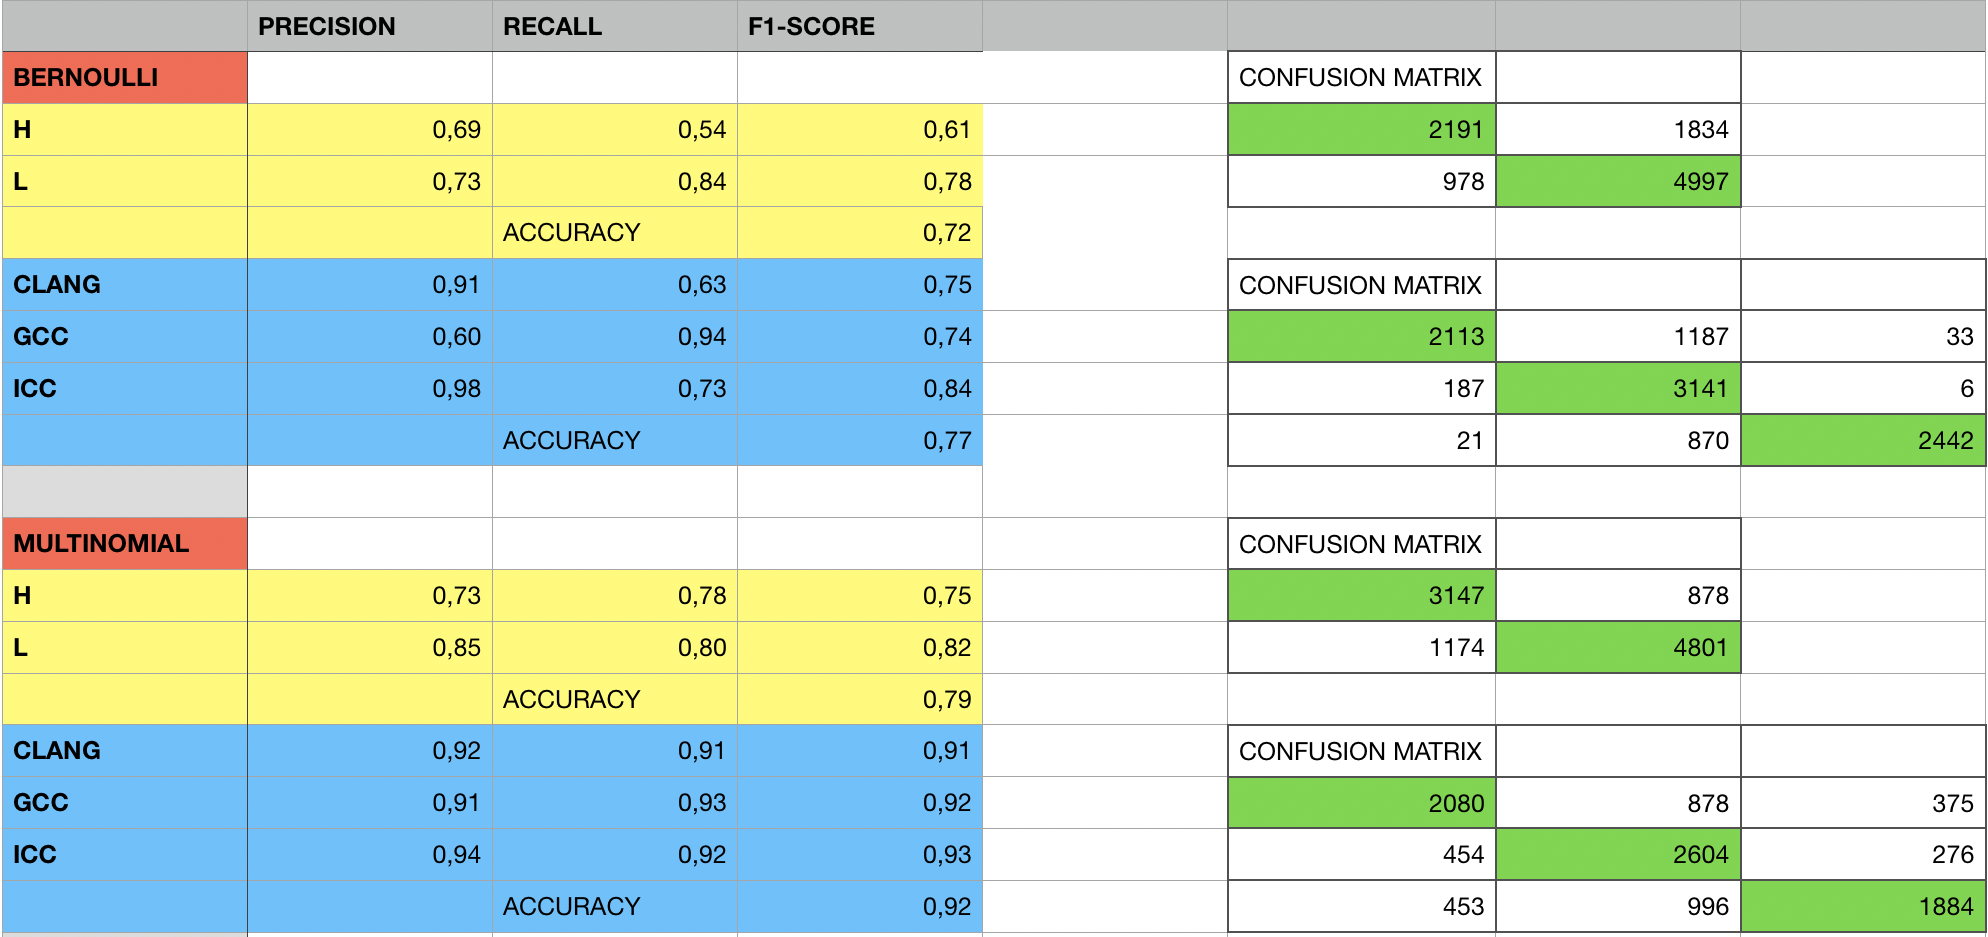
\includegraphics[width=1\textwidth]{pic5}
 \label{fig: Bernoulli and Multinomial with 3-grams}
\end{figure}

As we can see with BernoulliNB and 3-grams we slightly improve our result but as we expected with MultinomialNB the results start to be good. Analyze it.
About the compiler detection, we have an accuracy of 0,92 and this is a really good result because it ensures a low value for the FPR. Instead, for optimization detection, the result is still a bit low. We report below the FP-rate and FN-rate and we continue our analysis on these parameters because Precision and Recall can be easily related to FPR and FNR, indeed recall is simply 1 - FNR and the precision is higher with low FPR values.

\bigskip
\begin{tabular}{ | l | l | l | }
 \hline
 \textbf{Classes} & \textbf{FP-rate} & \textbf{FN-rate} \\ \hline
 H & 0,19648 & 0,21813 \\ \hline
 L & 0,21813 & 0,19648 \\ \hline
\end{tabular}
\bigskip

At this point, significative better results can be achieved only using a more sophisticated model and for this reason, we choose Linear Support Vector Machine.

\subsection{Linear SVM}
As a last attempt to improve our performances we use Support Vector Machine with Linear kernel, standard penalty parameter $C = 1$ and 3-grams. Goes to show the results.

\begin{figure}[!ht]
 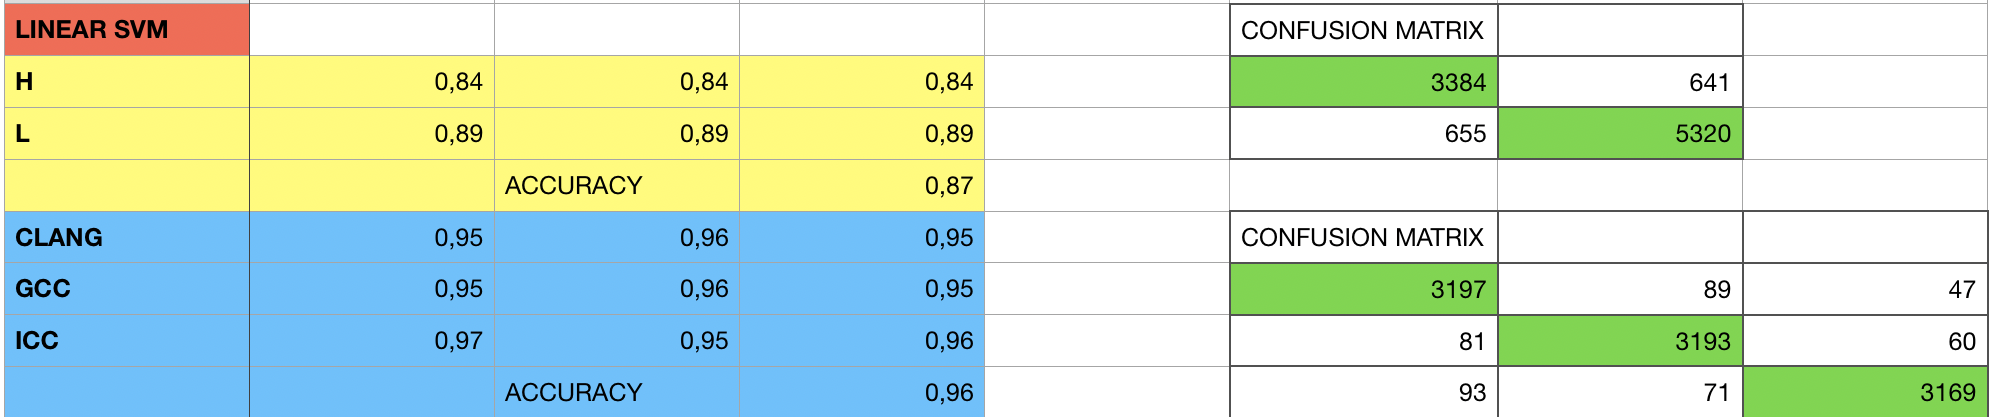
\includegraphics[width=1\textwidth]{pic6}
 \label{fig: Linear SVM with 3-grams}
\end{figure}

\bigskip
\begin{tabular}{ | l | l | l | }
 \hline
 \textbf{Classes} & \textbf{FP-rate} & \textbf{FN-rate} \\ \hline
 H & 0,10962 & 0,15925 \\ \hline
 L & 0,15925 & 0,10962 \\ \hline
 CLANG & 0,02609 & 0,04080 \\ \hline
 GCC & 0,02400 & 0,04229 \\ \hline
 ICC & 0,01604 & 0,04920 \\ \hline
\end{tabular}
\bigskip

Considering these measures, this model is for sure the best than the others, indeed, we have improved the compiler detection performance even more, but the most convincing result is the fact that we have increased the optimization detection rates bringing them to much better values. As you can see we have taken the FPR from 0.19 to 0.10 for H and from 0.21 to 0.15 for L.

At this point, we finish our analysis here and we can draw our conclusions.

\section{Conclusion}
From these results we could see the fact that SVM is certainly one of the best models, therefore continue to test other models probably wouldn't be worth it. The thing that surely can improve our results, even more, is the extraction of features. Indeed, in the beginning, we showed that we based our analysis only perform the mnemonics of function and the memory and register accesses. Surely by investigating more about the behavior of the various compilers and the many assembly instructions we could find better solutions. For now, we end our experience here.

Note that we perform the {\em Blind-dataset} with the last combination: Linear SVM with 3-grams.

\vfill

\begin{thebibliography}{99}

\bibitem{wiki}
{\em SKlearn Documentation}. 
 \verb|https://scikit-learn.org/stable/documentation.html|

\bibitem{nist}
C. Bishop
 {\em Pattern Recognition and Machine Learning}.

 \bibitem{nist}
{\em Wikipedia - Tf-Idf}.
 \verb|https://en.wikipedia.org/wiki/Tf–idf|

\end{thebibliography}
\end{document}